\documentclass[oneside, 12pt]{memoir}
\usepackage{verbatim}
\usepackage[labelsep=period, font=singlespacing, skip=12pt, format=hang, justification=RaggedRight, singlelinecheck=false]{caption}
\usepackage[T1]{fontenc}
\usepackage{times}
\usepackage{indentfirst}
\usepackage{thesis}
\usepackage{frontmattercontents}
\usepackage{listings}
\usepackage{graphicx}
\usepackage{hyperref}
\usepackage{layouts}

\graphicspath{{./images/}}

\lstset{ %
xleftmargin=.2in,
xrightmargin=.1in,
language=Python,                	% choose the language of the code
basicstyle=\footnotesize,       % the size of the fonts that are used for the code
numbers=left,                   % where to put the line-numbers
numberstyle=\footnotesize,      % the size of the fonts that are used for the line-numbers
stepnumber=2,                   % the step between two line-numbers. If it's 1 each line 
                                % will be numbered                                                         
numbersep=5pt,                  % how far the line-numbers are from the code
showspaces=false,               % show spaces adding particular underscores
showstringspaces=false,         % underline spaces within strings
showtabs=false,                 % show tabs within strings adding particular underscores
frame=single,	                % adds a frame around the code
tabsize=2,	                	% sets default tabsize to 2 spaces
captionpos=b,                   % sets the caption-position to bottom
breaklines=true,                % sets automatic line breaking
breakatwhitespace=false,        % sets if automatic breaks should only happen at whitespace
title=\lstname,                 % show the filename of files included with \lstinputlisting;
                                % also try caption instead of title
escapeinside={\%*}{*)},         % if you want to add a comment within your code
morekeywords={*,...}            % if you want to add more keywords to the set
}


\checkandfixthelayout
\begin{document} 
	\setdoctype{Polemic}
	\masters 
	
	
\settitle{Modeling Mobile Web Characteristics for Energy Optimized Delivery}
\setauthor{Troy Johnson}

\setdefdate{September 2014}
\setgraddate{December, 2015}

\setchair{Dr. Patrick Seeling, Ph.D.}
\setmembers{Dr. Patrick Kinnicutt, Ph.D. \\ Dr. Michael Stinson, Ph.D.}


\newcommand{\titlepage}{{
\clearpage
\thispagestyle{empty}

\begin{SingleSpace}
\centering
\cmutitle \\
\vspace{1.42in} 
\cmuauthor \\
\vspace{1.42in}
A thesis submitted in partial fulfillment of\\
the requirements for the degree of\\
Master of Science \\
\vspace{2.333in}
Department of Computer Science \\
\vspace{2in}
Central Michigan University\\
Mount Pleasant, Michigan \\
September 2014\\
\end{SingleSpace}
\clearpage}}


\newcommand{\signaturepage}{{
\clearpage
\thispagestyle{plain}
{\centering
Accepted by the Faculty of the College of Graduate Studies,\\
Central Michigan University, in partial fulfillment of\\
the requirements for the master's degree\\}
\vspace{12pt}
{\noindent
Thesis Committee:\\}
\setlength{\tabcolsep}{0mm}
\begin{tabular}{{@{}l @{\hspace{10mm}}l}}
\rule{92mm}{.3pt}  &  Dr. Patrick Seeling \\
\rule{92mm}{.3pt}  &  Dr. Patrick Kinnicutt \\
\rule{92mm}{.3pt}  &  Dr. Michael Stinson \\
Date: \rule{81mm}{.3pt} & \\
\rule{92mm}{.3pt}  &  Dean \\ 
Date: \rule{81mm}{.3pt} & \parbox[tl]{2in}{\vspace*{-32pt} College of Graduate Studies} \\
\end{tabular}\\

{\noindent
Committee:\\
 
}
\clearpage}}

\newcommand{\acknowledgementspage}{{%
\clearpage
\thispagestyle{plain}

{\centering
ACKNOWLEDGMENTS \\}
This work was sponsored by an Early Career Grant from the Office of Research and Sponsored Programs at Central Michigan University.
%\end{Spacing}
\clearpage}}


\newcommand{\abstractpage}{{
\clearpage
\thispagestyle{plain}

{\centering
ABSTRACT \\
\begin{SingleSpace}
\cmutitle \end{SingleSpace}
by Troy Johnson\\}

As mobile traffic and data consumption continue to rise, there is a growing need to investigate increased energy efficiency and optimizations to reduce the bandwidth when browsing the mobile web. Use cisco figure citations here???? To determine the reduction in energy consumption of mobile devices, there is also a need for a way to measure the energy consumption of mobile devices. By investigating the composition and characteristics of mobile web pages, statistical models can be derived for describing the characteristics of a typical mobile web page, such as the individual response sizes and expiration ages of responses that mobile browsers request for web pages.HTTP Archive will be a great source of data that may be utilized to derive models for describing the mobile web. Additionally, this pool of data is updated on a bimonthly basis, providing a constantly updated pool of data to update the developed models with and validate them. These models can then in turn be used to provide more accurate results when estimating the possible energy and bandwidth savings by using these models for generating artificial web pages that will contain characteristics that closely resemble those characteristics often found on the actual mobile web.  Investigating the models and data further, they can be extended to create prediction models that will describe the growing mobile web for future years. With these models in place, they can be applied to projects for optimizing energy and bandwidth consumption on mobile devices, such as the possible energy and bandwidth savings that can result from cache forwarding between desktop computers and mobile devices. To measure the possible energy consumption savings from these projects, a low cost test bed for measuring the power consumption of mobile devices can be employed as a baseline
\clearpage}}

	

\frontmatter
\setulmarginsandblock{0.75in}{1.25in}{*}
\titlepage
\clearpage
\pagebreak
\begin{Spacing}{2}
\acknowledgementspage
\clearpage
\pagebreak
\abstractpage
\clearpage
\pagebreak
\tableofcontents*
\clearpage
\pagebreak
\listoffigures
\clearpage
\pagebreak
\pagestyle{plain}
\checkandfixthelayout
\mainmatter
\counterwithout{figure}{chapter}
\addtocontents{toc}{\noindent CHAPTER \par}
\setulmarginsandblock{0.75in}{1.25in}{*} 


\chapter{INTRODUCTION}

\subsection{HTTP Archive}
HTTP Archive is an online repository of web performance information containing information on both desktop and mobile versions of websites. Information gather includes all the details about the responses each webpage makes such as the response sizes, expiration age, HTTP Archive gathers their data using a private instance of WebPageTest [CITATION????]. 

%Notes: Add more description in demonstration section
%Pull more specifics from the powepoint, also more
%description on the proxy overhead paper
\chapter{An Inexpensive Testbed for Mobile Device Power Measurement} 
\label{ch:testbed}


\section*{Introduction}
%addcontentsline add section to table of contents
\addcontentsline{toc}{section}{Introduction}

Over the last few decades, there has been an enormous increase in the ubiquity of mobile devices. With this increase, has also come the increase in demand for data-driven services and this demand is predicted to continue \cite{VNI14}. The battery consumption of mobile devices represents a limiting bottleneck and thus  power optimizations suggestiosn have been suggested \cite{Qian:2012:PTM:2187836.2187844}. Software-based energy profilers do exist \cite{DAmato:2011:EAE:2419622.2419929}, however they are not always feasible for implementing in a straightforward manner or desirable due to rapid development cycles. To overcome these barriers, a real world test bed that can be implemented which to perform measurement of power consumptions on mobile devices.

\addcontentsline{toc}{section}{Hardware Configuration}
%Putting an asterisk after section leaves out the II. formatting
\section*{Hardware Configuration}

The main component in this testbed is the mobile device.
This can be realized by using a smartphone and replacing the
battery with connectors to the power supply; alternatively one
of the common development board packages, such as
Pandaboard (see www.pandaboard.org) or Wandboard (see
www.wandboard.org) packages. Development boards and smartphones were utilized together with the
Android operating system, which provides log output via USB
to the measurement control device, which can be a regular PC
or another development board with Android debugging
support. The mobile device is then networked with a wireless access point, which allows for wired and wireless evaluations.
The switchable power supply has an external serial or USB
port to communicate the current and power in small time
intervals to the control device. A BK Precision
1696 switchable power supply is utilized, as it offers fine granularity in power, current, and time intervals. While other equipment, such as Arduino with custom circuits, were used in other measurement approaches, these power supplies are common lab equipment and offer overall robust features.

\addcontentsline{toc}{section}{Software Configuration}
\section*{Software Configuration}
The software components are comprised of several Python scripts that execute the Android Debugging Bridge (ADB) and capture the output either to a local file or allow sending the output to a remote receiver, as illustrated in  Figure \ref{fig:testbed_setup}. The scripts allow for easy customization on the locally connected control device or at a remote location, e.g., filtering by specific events in the log. Similarly, a locally executing script captures the output from the power supply and is enabled to forward the data to a remote location as well.

\begin{figure}
\centering
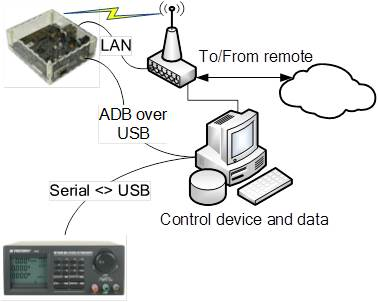
\includegraphics[scale=1,keepaspectratio]{testbed_setup}
\caption{Illustration of measurement testbed.}
\label{fig:testbed_setup}
\end{figure}

\addcontentsline{toc}{section}{Demonstration Description}
\section*{Demonstration Description}
To demonstrate the usefulness of the testbed, two different aspects of the measurement setup were utilized using an example Android application that performs web requests. This application makes requests to a local proxy server either serially or in parallel and the proxy server goes out and fetches what the phone requested.  The workflow for the application ca be seen in figure \ref{fig:testapp_workflow}. Both, wired and wireless access scenarios were exhibited for accessing a remote web service and retrieving results in order to demonstrate the functionality of the testbed. With these demonstrations, real time visualizations of the data about power consumption were created and stored on log files on a remote computer where they can be readily parsed for automatic evaluation  of application power consumption.

\begin{figure}
\centering
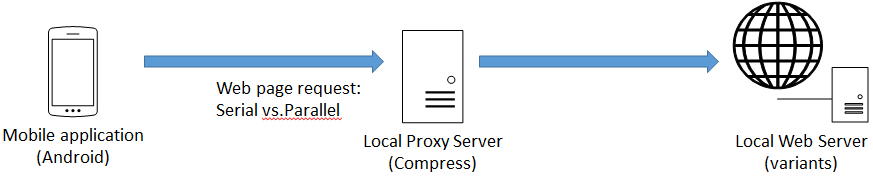
\includegraphics[scale=1,keepaspectratio,width=\textwidth]{testapp_workflow}
\caption{Workflow of mobile application tested on testbed.}
\label{fig:testapp_workflow}
\end{figure}

%Notes:Talk about what exactly a proxy server is
\chapter{Power Consumption Overhead for Proxy Services on Mobile Device Platforms}
\addcontentsline{toc}{section}{Introduction}
\section*{Introduction}
Current predictions by Cisco show that the amount of data that users consume has increased significantly and will continue to increase into the foreseeable future \cite{VNI14}. Previous studies show that the network interfaces of mobile devices consume much of the limited battery life \cite{Carroll:2010:APC:1855840.1855861}. Thus, heavy research efforts have been poured into studying the possibilities of energy efficient mobile data delivery. Some research avenues have middleware that acts as an on-device proxy service to realize benefits or enable new interaction paradigms, such as display networks \cite{6174992} or mobile content sharing \cite{Seeling:2014:OES:2671189.2671194},\cite{6692468}. To determine whether or not these local proxy servers result in a large overhead in terms of power consumption and time delays, the measurement framework testbed described in Chapter \ref{ch:testbed} can be implemented to determine what kind of overheads can be expected from local proxy servers. 

\chapter{CONCLUSION}

	
\subsection*{Future Work}
\addcontentsline{toc}{subsection}{Future Work}



\end{Spacing}
\bibliographystyle{unsrt}
\bibliography{main}
\end{document}
